% !TeX root = ../dissertation.tex

\newcommand{\codeat}[1]{\normalfont{\small Code at \texttt{#1}}}

\newcommand{\codesection}[2]{
      \section[#1]{#1\\\codeat{#2}}
}
\newcommand{\codesubsection}[2]{
      \subsection[#1]{#1\\\codeat{#2}}
}
\newcommand{\codesubsubsection}[2]{
      \subsubsection[#1]{#1\\\codeat{#2}}
}

\chapter{Implementation}

\codesection{Architectual Overview}{src/rust/ocaml-jis-shared/src/instructions/types.rs}

Test

\codesubsection{Architectual Overview}{src/rust/ocaml-jis-shared/src/instructions/types.rs}

Test

\codesubsubsection{Architectual Overview}{src/rust/ocaml-jis-shared/src/instructions/types.rs}

Test

\section{Development methodology}

\section{Instruction parsing}

\subsection{Types}

Maybe I should talk about the Instruction type that gets used everywhere

\subsection{Parser}

\section{The initial compiler}

There were two milestones in the project where the initial compiler was complete: after the
implementation of the initial compiler and after the integration with the optimising compiler. The
essential difference between them is the addition of a level of pointer indirection at function
calls to allow patching the address of a function after it has been optimised.

I will describe the first implementation in this section and describe the modifications made to
support dynamic recompilation in the subsequent section REF.

\subsection{Overview of design}

In order to ensure correctness, the initial compiler produces assembly with \emph{exactly the same
      semantics} as the interpreter does (with minor exceptions covered later). The exact same
operations
are performed in the same order as the bytecode running in the interpreter performs.

The only difference is rather than use bytecode, the operations are inlined into direct assembly.
Bytecode branches are translated to machine code branches. There are two reasons why it is
reasonable to expect this to be faster:

\begin{enumerate}
      \item This design integrates much better into the instruction pipelines, branch prediction
            and
            out-of-order execution modern CPUs are capable of
      \item Operands can be hard-coded into the machine code rather than requiring another memory
            lookup. For example, rather than performing generalised pointer addition when looking
            up
            a field
            the exact offset can be included in the addressing mode.
\end{enumerate}

\subsection{Main library used}

The project makes use of the \texttt{dynasm-rs} library. The design of this library allows for
writing assembly code snippets in the source code. The assembly is validated and mostly assembled
at compile time using Rust procedural macros and a much smaller runtime library deals with any
relocations and labels.

This library was a great success as it allowed me to operate at the level of the library without
being concerned about how the assembly maps to binary. The ahead-of-time aspects means there was
very little overhead at runtime - much less than alternative approaches like making an assembly
builder or printing assembly and forking out to an assembler would use.

\subsection{Mapping of the abstract machine}

The first compiler uses a fairly direct translation from OCaml bytecode to assembly.

The x86\_64 registers \texttt{r12-r15} (callee-saved in the System V calling convention) are used
to store the OCaml registers - however the system PC is used instead of the bytecode pointer.

\subsection{Implementation overview}

\subsection{Further details}

The above explanation is an over-simplification. Here is an non-exhaustive list of complicating
factors:

\subsection{Implementation strategy}

Implementation followed an incremental and highly test-driven strategy over multiple weeks. The
initial focus was on building a system sophisticated enough to run a hello world program
implementing the bare minimum instructions to support this.

I then slowly expanded the complexity of programs using them to drive the implementation of new
instructions and the fixing of bugs in the previous programs.

As is mostly inevitable in a project of this complexity hand-writing assembly there were a
significant number of bugs. Traditional debugging methods like print debugging or using a debugger
could not be as easily applied. Some errors resulted in confusing segfaults without any clear
indication
of what went wrong (although by poking around in the memory with GDB I was able to fix them).

Despite this the actual implementation was remarkably efficient. This is mainly due to the trace
comparison tooling I developed at the very start of the project and continued to expand throughout
the project.

\subsection{Trace comparison} \label{tracing}

There is no formal specification for the OCaml interpeter. The semantics of the interpreter are
what
\texttt{interp.c} and other files in the runtime say they are. Given this I decided to build
tooling to test the behaviour of my JIT-compiled code directly against the behaviour of the
interpreter.

\subsubsection{Tracing}

In order to do this I added support for tracing after every instruction in both the existing
interpreter and the JIT-compiled code. The log entry contains the instruction executed, state of
all of the OCaml registers and the top 5 entries on the stack.

There are a few log formats that it can print - for this application I used \texttt{serde} to
serialize and deserialize the trace entries as JSON. The trace comparison program launches the
program: once with the interpreter and once using the JITed code

\subsubsection{Comparison}

A wrapper program (in the \texttt{ocaml-jit-tools} crate) runs a sepcified program with
tracing enabled twice simultaneously - one run uses the JIT and the other the
existing interpreter.

Then for every trace entry received it compares the two lines. If there is a difference between the
lines
it shows a diff and then exits.

As many of the values are pointers there is a risk of non-determinism making this comparison fail.
I used a small wrapper program I found caled \texttt{no-aslr} to disable ASLR. In order to ensure
that the Rust code doesn't cause them to become unaligned I ran the compiler regardless of whether
JITed code was enabled when tracing was enabled. These two things together worked well enough that
all of the memory addresses were aligned and deterministic. This is unlikely to be true in general
for all OS kernels and malloc implemenations but worked for me.

The only expected difference comes from the use of the machine PC rather than the bytecode PC -
instruction pointers like return addresses on the stack could differ. This required a special case
during the check.

I added a script to run about 10 test programs that together mostly covered the entire instruction
set. Running this frequently allowed me to test for regressions when making changes.

\subsection{Towards full correctness}

Once I was happy that I had implemented every instruction, I started using
the OCaml compiler's internal test suite. I discovered some subtle bugs and used it to add new test
programs and fix them by trace comparison. One test heavily used callbacks from C to OCaml and I
discovered my initial implementation was too slow.

I eventually managed to get nearly all tests in the test suite working - the only failures were
testing the backtrace support and the debugger.

After this I successfuly managed to bootstrap the compiler using the JIT which gave me a high level
of confidence in the accuracy of the JIT-compiled code.

\subsection{Next steps}

The next steps were to add the benchmark suite. More detail is given later in the evaluation
chapter but the summary is the results were good and validated that this approach could be
performant. I had some time left to work on significant extensions.

\subsubsection{Initial plan and SSA form}

I noticed from looking at the structure of the compiled code that a large source of inefficiency
was the reliance on the stack machine model. This made nearly every operation involve reading from
or pushing to memory and made little use of hardware registers. Values would be pushed to memory
only to be dropped by a \texttt{Pop} operation later and all function arguments needed to be placed
on the stack.

To futher investigate the feasibility of doing something more feasible I decided to produce a
system which would parse the bytecode into an SSA-type intermediate representation where the OCaml
stack or accumulator registers were not explicitly used. To test this idea in isolation I decided
to develop it as a dissasembler. The output of the dissasembler is GraphViz \texttt{dot} files for
each functions which are converted into hyperlinked \texttt{svg} files.

The final version of the optimised compiler did the same conversion from explicit stack to implicit
stack with SSA but performed it in a different way. The reasons for these differences are explained
later in section REF. However the code still appears in the final deliverable as part of the
`clever' dissasembler.

\subsubsection{Optimised compiler}

Having developed this SSA form I had two choices for how to proceed.

\begin{enumerate}
      \item write an x86\_64 compiler backend from scratch
      \item use a compiler framework to do the translation from an IR that is closer in semantics
            to
            the existing SSA
\end{enumerate}

With the limited time remaining and considering the scope of the project I decided that the first
option was infeasible. For the second, the typical choice to use is LLVM. LLVM is developed by
Apple and used to support many languages and compilers including Rust, Swift and Clang for C.
Although typically used for ahead-of-time compilation it has support for use in JIT compilation. It
additionally contains some support for garbage collection including a model that can be used for
safepoints.

I initially decided to go with LLVM but as the implementation started I ran into some limitations.

\begin{itemize}
      \item LLVM is very large and bloated - compiling it with multiple jobs caused my machine to
            run
            out of memory and linking it in massively bloated the binary size of \texttt{ocamlrun}
      \item The safepoint GC support while somewhat mature is messy and would require writing
            patching the C++ source of LLVM to add new options as well as diving very deep into
            internal data
            structures
      \item LLVM has about 2 different JIT interfaces (\texttt{MCJit}, \texttt{orc},
            \texttt{orc1}),
            all of which had different limitations when used in a project such as mine
      \item Although there are some very good Rust bindings, not all features of the C++ api are
            exposed. This is especially true with the garbage collector support.
      \item LLVM is somewhat heavyweight and slow to compile which makes it inherently less well
            suited for use in this project
\end{itemize}

It was at this point that I discovered the \texttt{cranelift} project which seemed in many ways to
be exactly what I needed.

\begin{itemize}
      \item It is written in Rust which means the API is fairly idiomatic when using it in Rust
      \item It is designed primarily for JITs and focuses heavily on compilation performance
      \item The project is actively developed and I could communicate with the developers when I
            had
            questions who were very responsive.
      \item Although the support for garbage collection is not as extensible, with the help of the
            developers I was able to come up with a model that is a good fit for the OCaml garbage
            collector's
            requirements.
      \item When I encountered any bugs or missing features I could easily submit and get merged
            patches to the project which uses a familiar Github workflow rathter than the LLVM
            project's legacy
            systems.
\end{itemize}

There were still some missing features in Cranelift which are described later but for the most
part it was a good fit for my needs and was in a large part responsible for my being able to
finish this project in time.

\section{Modifications to support dynamic recompilation}

\subsection{Closure metadata table}

OCaml closures consist of a heap-allocated block containing a code pointer and the closure env
variables. In the original interpreter this code pointer pointed at a bytecode instruction. In this
second this was replaced with a pointer to the machine code.

However, different closures can use the same code pionter. The optimsed compiler optimises the code
in isolation rather than the specific instance in the closure. We also need to keep a count of the
number of times a section of code is executed to know when to branch into the compiler.

To do these tasks, I extended the initial compiler to have a pass to discover all of the closures
referenced in the program. For each of these I allocate a 32 byte entry in a table and modified the
code pointers in closusres to point to these values.

The format of this is INCLUDE THE FORMAT HERE.

\subsection{Transforming partially to eval-apply}

As described in section REFTODO, the OCaml interpreter uses a push-enter model for function calls.
Projects like Cranelift and LLVM tend to use a calling model which is closer to that of C to
support the platform ABI. This is also what the CPUs themseleves are optimsed to do.

For this reason I decided to convert from the push-enter model (callee deals with arity mismatch)
to an eval-apply model (caller deals with arity mismatch).

There is already some shared tasks performed on every apply - checking for stack resizing and
checking signals. I modified every apply in such a way that dealing with

For simplicity, I only decided to support the optimisation of functions taking 5 or fewer arguments
which is the vast majority of them. Arguments are passed according to the C calling convention with
the closure environment always passed as the first argument.

\textbf{MENTION needing to support optimised calls from cranelifted to cranelifted}

\section{Optimised compiler}

\subsection{Cranelift design}

Cranelift is a THING similar to LLVM.

This means that a goal is to have a mostly target-independent format which can be shared between
the backends.

Cranelift IR is in SSA. In order to make this easier to use cranelift includes an online IR builder
based on the work of LINKPAPERFORCRANELIFTSHIT.

Unlike LLVM, cranelift uses block parameters rather than Phi nodes. Link to the paper. In practice,
this is a slightly nicer model to work with.

Cranelift is a typed IR with integer types, functions and crucially for our needs reference types.
These were originally created to support webaseembly reference types whose garbage collection uses
reference counting but it's fully precise (DEFINE) nature means it can be used to fit our needs.

\subsection{The optimised compiler}

The steps taken are

\begin{enumerate}
      \item Convert the instructions into basic blocks and analyse stack starts
      \item Translate each basic block into Cranelift instructions using cranelift variables to
            deal
            with variable positions
      \item Run cranelift on the source
      \item Store stack maps emitted by cranelift in the hashmap for garbage collection
\end{enumerate}

\subsection{Basic block conversion and stack starts}

The compiler starts by parsing the instructions into basic block instructions. The algorithm is
essentially a depth first search where the stack pointer is updated.

Give pseudo-code for the search

Once this is done we are ready to convert the basic blocks to the form that cranelift expects.

\subsection{Conversion to Cranelift IR}

The structure of this is remarkably similar to the interpreter, and the original compiler. The only
difference is rather than pushing and popping.

Cranelift works with the concept of an IR builder which is based around the core Value type. For
example \texttt{2 + 3} might naively be translated into this sequence of calls

\begin{minted}{rust}
let av = self.builder.ins().iconst(types::I64, 2); // av : Value
let bv = self.builder.ins().iconst(types::I64, 3); // bv : value
let result = self.builder.ins().iadd(av, bv);      // result: Value
\end{minted}

\section{Trace comparison for the Cranelift compiler}

In order to have any hope of creating a correct mapping for cranelift code to

Talk about apply tracing using the existing compiler as the gold standard

\subsection{Garbage collection support}

Talk about R64 and I64 types, conversion between them and what Cranelift does RE spilling and stack
slots

\subsubsection{Unwinding with \texttt{libunwind}}

Talk about problems with using libunwind and generic DWARF debug info

\subsubsection{\texttt{rbp} unwinding}

Compiling with no emit frame pointer made this much easier

\subsubsection{Final design}

\subsection{Bigger picture}

test

\section{Disassembly tools}

\subsection{SSA dissassembler}

\subsubsection{Unifying stack variables}

\subsubsection{Parsing debug info}

\section{Overview of repository}

\dirtree{%
      .1 /.
      .2 benchmarks.
      .3 sandmark\DTcomment{fork of the Sandmark benchmark suite to support bytecode}.
      .3 analysis\DTcomment{Jupyter notebooks analysing benchmark results}.
      .2 docs\DTcomment{{\LaTeX} source of proposal, report and this document}.
      .2 scripts\DTcomment{scripts to run tests and graph basic blocks}.
      .3 run\_tests.sh\DTcomment{runs the entire suite of benchmark tests}.
      .2 src.
      .3 rust.
      .4 ocaml-jit-shared\DTcomment{shared library between the other two crates}.
      .4 ocaml-jit-staticlib\DTcomment{crate linked in to OCaml runtime}.
      .4 ocaml-jit-tools\DTcomment{standalone tools used for testing}.
      .3 ocaml\DTcomment{contains a fork of the entire OCaml compiler}.
      .4 runtime\DTcomment{where most modifications to the OCaml compiler happened}.
      .5 jit\_support.c\DTcomment{contains C primitives used by the compiled code}.
      .3 vendor\DTcomment{contains forked Rust dependencies}.
      .2 test-programs\DTcomment{OCaml source for the test programs used by the scripts}.
      .2 no-aslr\DTcomment{A simple wrapper to run a program without ASLR}.
}

\subsection{ocaml-jit-shared crate}

\dirtree{%
      .1 src/rust/ocaml-jit-shared.
      .2 Cargo.toml\DTcomment{specifies dependencies}.
      .2 src.
      .3 basic\_blocks\DTcomment{contains types and algorithm for converting an instruction stream
            to
            basic blocks}.
      .3 cranelift\_compiler.
      .4 mod.rs\DTcomment{Contains the bulk of the implementation of the optimised compiler}.
      .4 test\_cases\DTcomment{Contains many expect-test cases}.
      .3 instructions.
      .4 parse.rs\DTcomment{contains the parser for OCaml bytecode}.
      .4 types.rs\DTcomment{defines the core instruction types used everywhere}.
}

\subsection{ocaml-jit-staticlib crate}

\dirtree{%
      .1 src/rust/ocaml-jit-staticlib.
      .2 Cargo.toml\DTcomment{specifies dependencies}.
      .2 src.
      .3 caml\DTcomment{contains Rust wrappers for OCaml headers}.
      .3 compiler.
      .4 c\_primitives.rs\DTcomment{imports C primitives from the OCaml runtime}.
      .4 emit\_code.rs\DTcomment{contains the bulk of the implementation of the initial compiler}.
      .4 rust\_primitives.rs\DTcomment{contains primitives written in Rust called by JITed code}.
      .4 saved\_data.rs\DTcomment{defines the persistent data structures the compiler adds}.
      .3 c\_entrypoints.rs\DTcomment{glue for C to Rust FFI}.
      .3 configuration.rs\DTcomment{defines the env-var options the JIT has}.
      .3 lib.rs\DTcomment{contains the entrypoints into the Rust code}.
}

\section{Architectural overview}


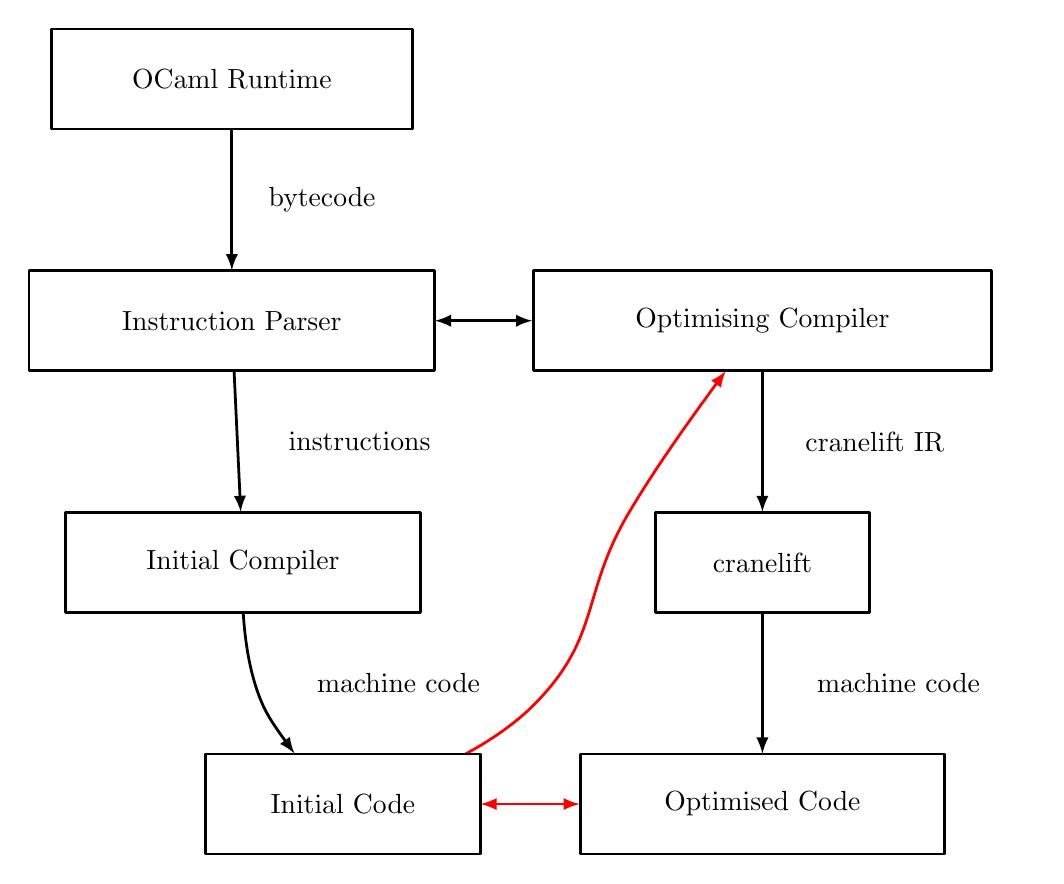
\begin{tikzpicture}[>=latex,line join=bevel,]
  \pgfsetlinewidth{1bp}
%%
\begin{scope}
  \pgfsetstrokecolor{black}
  \definecolor{strokecol}{rgb}{1.0,1.0,1.0};
  \pgfsetstrokecolor{strokecol}
  \definecolor{fillcol}{rgb}{1.0,1.0,1.0};
  \pgfsetfillcolor{fillcol}
  \filldraw (0.0bp,0.0bp) -- (0.0bp,297.0bp) -- (362.0bp,297.0bp) -- (362.0bp,0.0bp) -- cycle;
\end{scope}
\begin{scope}
  \pgfsetstrokecolor{black}
  \definecolor{strokecol}{rgb}{1.0,1.0,1.0};
  \pgfsetstrokecolor{strokecol}
  \definecolor{fillcol}{rgb}{1.0,1.0,1.0};
  \pgfsetfillcolor{fillcol}
  \filldraw (0.0bp,0.0bp) -- (0.0bp,297.0bp) -- (362.0bp,297.0bp) -- (362.0bp,0.0bp) -- cycle;
\end{scope}
\begin{scope}
  \pgfsetstrokecolor{black}
  \definecolor{strokecol}{rgb}{1.0,1.0,1.0};
  \pgfsetstrokecolor{strokecol}
  \definecolor{fillcol}{rgb}{1.0,1.0,1.0};
  \pgfsetfillcolor{fillcol}
  \filldraw (0.0bp,0.0bp) -- (0.0bp,297.0bp) -- (362.0bp,297.0bp) -- (362.0bp,0.0bp) -- cycle;
\end{scope}
  \pgfsetcolor{black}
  % Edge: ocaml_runtime -> instruction_parser
  \draw [->] (73.0bp,260.8bp) .. controls (73.0bp,249.16bp) and (73.0bp,233.55bp)  .. (73.0bp,210.18bp);
  \definecolor{strokecol}{rgb}{0.0,0.0,0.0};
  \pgfsetstrokecolor{strokecol}
  \draw (105.5bp,235.5bp) node {bytecode};
  % Edge: instruction_parser -> optimising_compiler
  \draw [<->] (146.12bp,192.0bp) .. controls (161.16bp,192.0bp) and (166.08bp,192.0bp)  .. (181.11bp,192.0bp);
  % Edge: instruction_parser -> initial_compiler
  \draw [->] (73.809bp,173.8bp) .. controls (74.357bp,162.16bp) and (75.092bp,146.55bp)  .. (76.192bp,123.18bp);
  \draw (119.0bp,148.5bp) node {instructions};
  % Edge: optimising_compiler -> cranelift
  \draw [->] (264.0bp,173.8bp) .. controls (264.0bp,162.16bp) and (264.0bp,146.55bp)  .. (264.0bp,123.18bp);
  \draw (304.5bp,148.5bp) node {cranelift IR};
  % Edge: cranelift -> optimised_code
  \draw [->] (264.0bp,86.799bp) .. controls (264.0bp,75.163bp) and (264.0bp,59.548bp)  .. (264.0bp,36.175bp);
  \draw (313.0bp,61.5bp) node {machine code};
  % Edge: initial_compiler -> compiled_code
  \draw [->] (77.103bp,86.699bp) .. controls (77.721bp,76.765bp) and (79.471bp,64.265bp)  .. (84.0bp,54.0bp) .. controls (85.445bp,50.724bp) and (87.289bp,47.51bp)  .. (95.546bp,36.228bp);
  \draw (133.0bp,61.5bp) node {machine code};
  % Edge: compiled_code -> optimising_compiler
  \pgfsetcolor{red}
  \draw [->] (157.08bp,36.003bp) .. controls (166.06bp,40.865bp) and (174.92bp,46.835bp)  .. (182.0bp,54.0bp) .. controls (206.03bp,78.314bp) and (198.53bp,93.611bp)  .. (216.0bp,123.0bp) .. controls (224.7bp,137.63bp) and (235.56bp,153.2bp)  .. (250.79bp,173.89bp);
  % Edge: compiled_code -> optimised_code
  \draw [<->] (162.55bp,18.0bp) .. controls (177.79bp,18.0bp) and (182.99bp,18.0bp)  .. (198.21bp,18.0bp);
  % Node: instruction_parser
\begin{scope}
  \definecolor{strokecol}{rgb}{0.0,0.0,0.0};
  \pgfsetstrokecolor{strokecol}
  \draw (146.0bp,210.0bp) -- (0.0bp,210.0bp) -- (0.0bp,174.0bp) -- (146.0bp,174.0bp) -- cycle;
  \draw (73.0bp,192.0bp) node {Instruction Parser};
\end{scope}
  % Node: optimising_compiler
\begin{scope}
  \definecolor{strokecol}{rgb}{0.0,0.0,0.0};
  \pgfsetstrokecolor{strokecol}
  \draw (346.5bp,210.0bp) -- (181.5bp,210.0bp) -- (181.5bp,174.0bp) -- (346.5bp,174.0bp) -- cycle;
  \draw (264.0bp,192.0bp) node {Optimising Compiler};
\end{scope}
  % Node: cranelift
\begin{scope}
  \definecolor{strokecol}{rgb}{0.0,0.0,0.0};
  \pgfsetstrokecolor{strokecol}
  \draw (302.5bp,123.0bp) -- (225.5bp,123.0bp) -- (225.5bp,87.0bp) -- (302.5bp,87.0bp) -- cycle;
  \draw (264.0bp,105.0bp) node {cranelift};
\end{scope}
  % Node: initial_compiler
\begin{scope}
  \definecolor{strokecol}{rgb}{0.0,0.0,0.0};
  \pgfsetstrokecolor{strokecol}
  \draw (141.0bp,123.0bp) -- (13.0bp,123.0bp) -- (13.0bp,87.0bp) -- (141.0bp,87.0bp) -- cycle;
  \draw (77.0bp,105.0bp) node {Initial Compiler};
\end{scope}
  % Node: compiled_code
\begin{scope}
  \definecolor{strokecol}{rgb}{0.0,0.0,0.0};
  \pgfsetstrokecolor{strokecol}
  \draw (162.5bp,36.0bp) -- (63.5bp,36.0bp) -- (63.5bp,0.0bp) -- (162.5bp,0.0bp) -- cycle;
  \draw (113.0bp,18.0bp) node {Initial Code};
\end{scope}
  % Node: optimised_code
\begin{scope}
  \definecolor{strokecol}{rgb}{0.0,0.0,0.0};
  \pgfsetstrokecolor{strokecol}
  \draw (329.5bp,36.0bp) -- (198.5bp,36.0bp) -- (198.5bp,0.0bp) -- (329.5bp,0.0bp) -- cycle;
  \draw (264.0bp,18.0bp) node {Optimised Code};
\end{scope}
  % Node: ocaml_runtime
\begin{scope}
  \definecolor{strokecol}{rgb}{0.0,0.0,0.0};
  \pgfsetstrokecolor{strokecol}
  \draw (138.0bp,297.0bp) -- (8.0bp,297.0bp) -- (8.0bp,261.0bp) -- (138.0bp,261.0bp) -- cycle;
  \draw (73.0bp,279.0bp) node {OCaml Runtime};
\end{scope}
%
\end{tikzpicture}



I have implemented a Rust static library which is linked in to the OCaml runtime library and
\texttt{ocamlrun} (the interpreter).
\texttt{ocamlrun} hooks into this library when it loads bytecode and when it starts
interpreting it.
If the JIT is enabled (either by setting an environment variable or enabling it by default at
compile time),
when the bytecode load hook is run the \textbf{initial compiler} will execute.

The initial compiler parses the bytecode into a stream of instructions and for each bytecode
instruction
it emits assembly with the same semantics to a buffer. After all code has been emitted (including
headers
and footers with shared routines) relocations are performed and the buffer is marked as executable.

When \texttt{ocamlrun} then calls the hook to start interpretation, the library instead jumps to
this assembly code which then performs the same operations as the interpreter - except that every
instruction has effectively been inlined.

When an OCaml closure is applied\footnote{all non-primitive function calls are translated to
      closure application}
a closure execution count is incremented. Once this count passes a configurable threshold the code
instead
branches in to the \textbf{optimising compiler}.

The optimising compiler operates on the level of a single function. It starts by doing a
depth-first search to discover all the basic blocks in the function. It then iterates over this
again producing Cranelift IR Format (CLIF) which is passed to the machinery of
\textbf{cranelift}. The CLIF code produced abstracts away the use of the stack allowing cranelift
to perform its register allocation. The function's code pointer is updated and any future calls
(including the originally triggering call) will use the optimised implementation.

\section{Major milestones}

The focus throughout all aspects of the project was focusing on working code that could be tested
even if the total wasn't complete. However it is worth noting the major milestones where some
degree of completeness was achieved. These entries are listed in chronological order.

\begin{enumerate}
      \item Execution of Hello World with the JIT
      \item Passing the OCaml test suite and bootstrapping the compiler
      \item Implementing the benchmark suite
      \item (Extension) Developing the advanced disassembler tools
      \item (Extension) Implementing the optimising compiler
\end{enumerate}

\section{Repository overview}

A more complete overview of the repository is given in section \ref{repo}. However, it is worth
drawing attention to which components are solely, partially or not at all my own work:

\dirtree{%
      .1 /.
      .2 benchmarks.
      .3 sandmark\DTcomment{fork of Sandmark with large patches}.
      .3 analysis\DTcomment{Jupyter notebooks analysing benchmark results}.
      .2 docs\DTcomment{{\LaTeX} source of proposal, report and this document}.
      .2 scripts\DTcomment{scripts to run tests and graph basic blocks}.
      .2 src.
      .3 rust.
      .4 ocaml-jit-shared\DTcomment{shared library between the other two crates}.
      .4 ocaml-jit-staticlib\DTcomment{crate linked in to OCaml runtime}.
      .4 ocaml-jit-tools\DTcomment{binary crate with standalone development/testing tools}.
      .3 ocaml\DTcomment{fork of OCaml compiler 4.11.1}.
      .4 runtime\DTcomment{contains most large patches for the JIT}.
      .3 vendor\DTcomment{vendored rust dependencies with small patches}.
      .2 test-programs\DTcomment{OCaml source for the test programs used by the scripts}.
      .2 vendor/no-aslr\DTcomment{A simple wrapper to run a program without ASLR}.
}

\section{Initial compiler}

The initial compiler was developed first before any work on the optimising compiler was done. In
the process of implementing the
initial compiler some modifications had to be made. These modifications will be covered later in
section \ref{dyn-recomp} and this section will mainly cover the initial state

\subsection{Overview}

The basic compiler consists of two larger components - an instruction parser and an assembly
emitter.

Most of the rest of the files are support for these components and deal with the FFI from and into
the existing runtime.

\subsubsection{Mapping of OCaml abstract machine}

The initial compiler operates by converting every bytecode instruction into a stream of assembly
instructions with the same semantics. Abstract machine registers are mapped to x86\_64 registers. A
pointer to the \texttt{Caml\_state} struct containing other global interpreter state is also
stored in a register called \texttt{r\_cs} for access to its fields with small code size. The
mapping used is shown in Table \ref{table:regmap}.

\begin{table}[h]
      \centering
      \begin{tabular}{cc}\toprule
            OCaml register          & x86\_64 register \\
            \midrule                                   \\
            \texttt{r\_env}         & \texttt{r12}     \\
            \texttt{r\_accu}        & \texttt{r13}     \\
            \texttt{r\_extra\_args} & \texttt{r14}     \\
            \texttt{r\_sp}          & \texttt{r15}     \\
            \texttt{r\_cs}          & \texttt{rbx}     \\
            \bottomrule
      \end{tabular}

      \caption{Mapping of OCaml to x86\_64 registers}
      \label{table:regmap}
\end{table}

Note that all x86\_64 registers mapped are callee-saved in the System V C calling convention. This
means that no work needs to be done spilling and restoring them from the C stack to call C/Rust
primitives (either as part of \texttt{CCall*} instructions or supporting primitives written for the
JIT).

\subsubsection{Mapping of the PC}

Bytecode pointers are mapped to native code pointers and the interpreter's PC is replaced with the
system's instruction pointer. This change is responsible for nearly all of the performance
improvements of the JITed code. The benefits are

\begin{itemize}
      \item Memory accesses are reduced - rather than loading operands and opcodes, they are baked
            in to the machine code
      \item The CPU can predict execution and fill its pipeline further than it can with the use of
            native code pointers
      \item Branch prediction in hot paths become more effective as each branch can be predicted
            differently
      \item Likewise, the CPU can schedule out-of-order execution more effectively across different
            instructions
\end{itemize}

However, this approach does lead to more contention on the instruction cache - rather than only
containing a single copy of the implementation of each instruction there are many.

\codesubsection{Hooks from OCaml}{src/rust/ocaml-jit-staticlib/src/c\_entrypoints.rs}

The existing OCaml runtime was modified to hook into the JIT at three points:

\begin{enumerate}
      \item After a bytecode section is loaded
      \item Before a bytecode section is released
      \item When the interpreter is called
\end{enumerate}

In most programs there are only 1\footnote{or 2 if callbacks from C to OCaml are used} sections
loaded. However, the interpreter is used in other places such as the toplevel REPL which motivates
the more general multiple section support.

Compilation happens after the first hook and an entry is written to a global table containing the
pointer to the buffer. The compiled code takes the form of a single large C function taking no
arguments.

When a section is released this entry is dropped which frees the memory.

The interpreter call hook then calls the JIT-compiled function representing that section.

\subsection{Instruction parsing}

The first stage in the pipeline is to parse the bytes into a stream of elements of the
\texttt{Instruction} type.

\codesubsubsection{The \texttt{Instruction}
      type}{src/rust/ocaml-jit-shared/src/instructions/types.rs}
\label{instruction-type}

OCaml has 149 opcodes, each of which can take different number of operands. Arguments and operands
are all stored as \texttt{i32} values. Rust has good support for algabreic sum types called enums
(which are much more general than the enums in a language like C).

Some of these opcodes are code-size optimisations which represent the composition of multiple
consecutive instructions or have a specific hard-coded operand value. For example,
\texttt{PUSHACC2} represents \texttt{PUSH} then \texttt{ACC2}. \texttt{ACC2} itself is a
specialisation of the more general \texttt{ACC(n)} instruction. These peephole-optimisation
enabling instructions make less sense for the purposes of our interpreter so only the simplest
instructions are considered.

Likewise, there are instructions like integer comparisons and conditional branches that have many
different variations changing only on the exact conditional used.

The instruction type is polymorphic over the type of the label to allow for different label
representations.

\codesubsubsection{Parser}{src/rust/ocaml-jit-shared/src/instruction/parse.rs}

The parser is implemented using Rust iterators; the parser takes an iterator of \texttt{i32}s and
produces an iterator producing values of type \texttt{Result<Instruction,
      ParseError>}\footnote{standard rust error handling type defined as \texttt{enum Result<T,E>
            \{Ok(T), Err(E)\}} like OCaml's \texttt{type ('a, 'b) result = Ok of 'a | Err of 'b}}.

This use of iterators makes the instruction parser consistently performant for large bytecodes -
consumers of the instruction stream take each instruction as they need it.

Labels are stored in the OCaml bytecode as indirect offsets relative to the current PC. To simplify
later uses, these are converted to absolute offsets relative to the start of the section.

As mentioned, single OCaml instructions may parse to more than one \texttt{Instruction}s. To
support this, the type contains a pseudo-instruction called \texttt{LabelDef} which is emitted at
the start of every OCaml instruction. This also allows building a map from OCaml bytecode
absolute offsets to parsed \texttt{Instruction}s.

\codesubsection{Code generation}{src/rust/ocaml-jit-staticlib/src/compiler/emit\_code.rs}

The code generation is the largest aspect of the compiler. It makes use of the \texttt{dynasm-rs}
library. This library manages emitting machine code and relocation information, relocating and
using \texttt{memmap} to mark the code as executable.

The compiler is triggered on the first time a `section' is loaded - for normal programs this is at
startup and for programs using the OCaml toplevel REPL this is after every statement is typed.

The compiler first emits a standard function header entrypoint which saves callee-saved registers
used by the compiler and aligns the C stack. A longjmp handler is set up for exceptions and then
for each bytecode instruction assembly with the same semantics is emitted.

During this process \texttt{dynasm-rs} dynamic labels are used to set up relocations: these
labels are defined before every bytecode instruction and can be referenced by any other
instruction. DynASM translates these at runtime into pc-relative jumps.

After all instructions are done, some shared code used by the instructions is emitted.
\texttt{dynasm-rs} then performs relocations and uses \texttt{mmap} to mark the region of code as
executable.

The overall signature of the assembly produced by this process is a single function taking no
arguments and returning an OCaml value. OCaml closure applications (function calls) do not produce
a stack frame on the C stack - the existing machinery using the OCaml stack is used instead.

\subsubsection{Simple example}

The main code of the compiler itself is contained in a 2000 line file
(\texttt{src/rust/ocaml-jit-staticlib/src/compiler/emit\_code.rs}). Most of this is taken up by a
Rust large pattern match for each of the bytecode instructions. As a very simple example of what
the code looks like consider the implemenation of the \texttt{Add} instruction. It adds the value
at the top of the OCaml stack to the accumulator and stores the result in the accumulator. Note
that the OCaml integer format means a decrement is required. In the original assembler it is
implemented as so:

\inputminted{c}{snippets/add.c}

In the compiler the case becomes:

\inputminted{rust}{snippets/add.rs}

This has exactly the same semantics. Note \texttt{r\_accu} and \texttt{r\_sp}
are aliases for \texttt{r13} and \texttt{r15}.

At compile time, the macro component of \texttt{dynasm-rs} translates it to:

\inputminted{rust}{snippets/add_comp.rs}

Most assembly work is done at compile time - the byte string above contains the machine code for
those instructions. This helps a lot with the performance of the compiler.

\subsubsection{Branches}

For example of the label and relocation support, consider the \texttt{BranchCmp(Comp, i32, L)}
instruction. It
compares the current value of the accumulator to the \texttt{i32} constant using the condition (of
type \texttt{enum Comp {Lt, Gt, ... }}). If the condition is true it branches to the label,
otherwise it passes to the next instruction.

This is implemented as so:

\inputminted{rust}{snippets/branchcmp.rs}

The macros translate it to:

\inputminted{rust}{snippets/branchcmp_comp.rs}

This shows the assembler work still needing to be done at compile time - relocations.

\subsubsection{Other cases}

Most other cases follow these patterns. Some more involved instructions will call into C primitives
I wrote instead (passing and then restoring the registers from the stack).

However, the basic structure of snippets of combined assembly and rust in a large pattern match
statement remains for all cases.

\subsection{Futher details}

Although the basic structure as described holds, some details are omitted but appear in
\texttt{emit\_code.rs}.

\begin{itemize}
      \item There is extensive optional support to support tracing instructions and events
            (described
            in section \ref{tracing})
      \item Callbacks from C to OCaml code require special handling
      \item The compiler returns a pointer to the first instruction to support OCaml's
            metaprogramming \texttt{ocaml\_reify\_bytecode} program used in the implementation of
            things like the
            toplevel \texttt{ocaml} program.
      \item Function application is a fairly involved process and there are checks to resize the
            stack and check for signals as well as the fundamental complexity of the push-enter
            model.
      \item Registers need to be saved and restored at safepoints to allow the garbage collector to
            use them
      \item Certain operations are involved enough that instead of inline the definition in
            hand-written assembly, I push the registers to the C stack and call a C primitive to
            implement the
            operation (taking the registers as a struct)
      \item The compiler stores a persistent data structure of the sections to allow mapping
            bytecode addresses to machine code addresses and allow for cleanup after a section is
            freed.
\end{itemize}

\section{Optimising compiler}

\subsection{Motivation and design}

Once the initial compiler was complete there was time to dedicate to a significant extension.
Although the initial compiler was performant, it lacked any optimisations between multiple
instructions.

The proposal lists a few ideas of extensions but does not commit to any one of them. Of these, the
decision made would be to focus on combining two concepts:

\begin{itemize}
      \item Dynamic recompilation of hot functions with more optimised forms
      \item Replacing the use of the stack with registers
\end{itemize}

The details of the first extension are explained later in section \ref{dyn-recomp} and the second
extension forms the basis of the optimised compiler the first extension calls.

The time left meant building a complete x86\_64 compiler backend (with register allocation,
instruction selection, etc.) from scratch was infeasible. The usual toolkit used to avoid
replicating this work is LLVM \cite{llvm}. Although is more typically known for its use in
ahead-of-time compilation, there is support for use in JITs.

\subsubsection{Problems with LLVM}

I initially decided to go with LLVM but as the implementation started I ran into some limitations.

\begin{itemize}
      \item LLVM is very large and bloated - compiling it with multiple jobs caused my machine to
            run out of memory and linking it in massively bloated the binary size of
            \texttt{ocamlrun}
      \item The safepoint GC support while somewhat mature is messy and would require writing
            patching the C++ source of LLVM to add new options as well as diving very deep into
            internal data
            structures
      \item Although there are some very good Rust bindings, not all features of the C++ api are
            exposed. This is especially true with the garbage collector support.
      \item LLVM has about 2 different JIT interfaces (\texttt{MCJit}, \texttt{orc},
            \texttt{orcv2}),
            all of which had different limitations when used in a project such as mine and only
            \texttt{MCJit} had good Rust bindings
      \item LLVM is somewhat heavyweight and compilation is slow which means there is a large risk
            of slower overall performance even if only compiling hot functions.
\end{itemize}

\subsubsection{Cranelift}

After struggling with these issues I discovered the \texttt{cranelift} project. Like LLVM it is a
retargetable code generator with an IR. However, it has a number of different design decisions
which made it much better suited for my planned uses:

\begin{itemize}
      \item It is written in Rust which means the API is fairly idiomatic when using it in Rust
      \item It is designed primarily for JITs and focuses heavily on compilation performance
      \item The project is actively developed and I could communicate with the developers when I
            had
            questions who were very responsive.
      \item Although the support for garbage collection is not as extensible, with the help of the
            developers I was able to come up with a model that is a good fit for the OCaml garbage
            collector's
            requirements.
      \item When I encountered any bugs or missing features I could easily submit and get merged
            patches to the project which uses a familiar Github workflow rathter than the LLVM
            project's legacy
            systems.
\end{itemize}

There were still some missing features in Cranelift which are described later but for the most
part it was a good fit for my needs and was in a large part responsible for my being able to
complete this ambitious extension.

\subsection{Overview}

At a high level is a function taking two inputs and returning two outputs. The inputs are a slice
to the code of a section, and the offset within that slice containing the first instruction in the
function to be optimised.

The first output is a pointer to a compiled function that can be called to execute the code
represented by that function. The second output is a vector of stack map entries which are used to
support finding GC roots (see section \ref{optgc}).

The compiler consists of three major components.

\begin{enumerate}
      \item Basic block conversion and stack start analysis (section \ref{opt-bb})
      \item IR generation from the basic blocks using the analysis (section \ref{opt-irgen})
      \item Compilation of IR to x86\_64 assembly
\end{enumerate}

The first two components are written by me and the third uses Cranelift.

As described later in section \ref{dyn-recomp}, this compiler is triggered once a function is
called enough times to become `hot'.

\codesubsection{Conversion to basic blocks}{src/rust/ocaml-jit-shared/src/basic\_blocks/}
\label{opt-bb}

The typical data structure used in optimising compilers is the basic block. \emph{Make sure I've
      defined this somewhere in preparation}.

However, the only information we have from the bytecode is a sequence of instructions with jumps.
In order to move away from a heavy connection with the instructions the first step is to decompile
to basic blocks.

\codesubsubsection{Types}{basic\_blocks/types.rs}

A \textbf{\texttt{BasicClosure}} consists of a vector of \textbf{\texttt{BasicBlock}} along with
some other data. A basic block has a vector of \textbf{\texttt{BasicBlockInstruction}} and a single
\textbf{\texttt{BasicBlockExit}}.

Some \texttt{Instruction}s (see section \ref{instruction-type}) map to a
\texttt{BasicBlockInstruction} and others map to a \texttt{BasicBlockExit}. For example,
\texttt{Instruction::Push} becomes \texttt{BasicBlockInstruction::Push} but
\texttt{Instruction::BranchIf(label)} becomes \texttt{BasicBlockExit::BranchIf { then\_block,
else\_block }}.

This enforces at the type level the basic invariant of basic blocks - one entry, one exit.

\subsubsection{Stack starts}

In addition to performing the conversion to basic blocks, the algorithm also keeps track of a
concept I call the \textbf{stack start} of a basic block. Although, like all other aspects of the
OCaml interpreter, it is not documented anywhere, inspecting the bytecode compiler's source and
testing against all real programs finds an important invariant:

For all paths leading from the entry block of a function to an instruction, the absolute stack size
relative to the start of the function's stack frame is the same.

During the conversion to basic blocks this invariant is validated and the size of the stack before
the first instruction of a block (the stack start) executes. This is the \textbf{stack start} of
the block.

\codesubsubsection{Algorithm}{basic\_blocks/conversion.rs}

The algorithm consists of two runs of DFS. The first finds all bytecode offsets which form the
start of blocks. The second visits all these blocks working out stack sizes.

In order to describe this algorithm without too many confusing details I will create a formalism
just complicated enough to include all the complexity.

The first DFS pass is only necessary to deal with loop back edges. For simplicity let's assume this
doesn't happen.

Let \(I\) be the set of all instructions. The program \(P\) is a list of instructions and can be
indexed. For simplicity, assume indices are consecutive\footnote{they're not but it's fairly simple
      to handle}.

Each instruction has four properties:

\begin{itemize}
      \item \(\delta(i)\) is the change to the stack pointer after executing the instruction. For
            example \texttt{Push} which pushes the acc to the stack has \(\delta(\texttt{Push}) =
            +1\)
      \item \(\dfsexit(i)\) returns \textbf{true} iff the instruction causes the block to end
            (jumps, returns)
      \item \(\dfsfallthrough(i)\) returns \textbf{true} iff \(\dfsexit(i)\) and it can end up
            jumping to the following instruction. \texttt{BranchIf(branch\_loc)} is fallthrough but
            \texttt{Branch(branch\_loc)} is not.
      \item \(\dfslabels(i)\) returns a set of all labels the instruction could end up jumping to
            (not
            including fallthrough). For example \(\dfslabels(\texttt{BranchIf(branch\_loc)}) =
            \{\text{branch\_loc}\}\). It is only relevant if \(\dfsexit(i)\)
\end{itemize}

Under this model, the algorithm to find all the blocks and their starts is shown in algorithm
\ref{alg-dfs}. The actual algorithm is more complicated and calculates more things but not
conceptually any different.

\begin{algorithm}
      \caption{DFS to find basic blocks and their starts}\label{alg-dfs}
      \begin{algorithmic}[1]
            \Function{FindBlocks}{$P, arity$}
            \State $seen \gets \emptyset$
            \State $starts \gets \{\}$
            \Function{VisitBlock}{$initial\_index, initial\_stack\_size$}
            \If{$initial\_index \in seen$}
            \Assert{$starts[initial\_index] = initial\_stack\_size$}
            \State \textbf{return}
            \EndIf
            \State $starts[initial\_index] \gets initial\_stack\_size$
            \State $i \gets initial\_index$
            \State $s \gets initial\_stack\_size$
            \Repeat
            \State $x \gets P[i]$
            \State $s \gets s + \delta(x)$
            \If{$\dfsexit(x)$}
            \For{$j \in \dfslabels(i)$}
            \State \Call{VisitBlock}{j, s}
            \EndFor
            \If{$\dfsfallthrough(x)$}
            \State \Call{VisitBlock}{i + 1, s}
            \EndIf
            \State \textbf{return}
            \Else
            \State $i \gets i + 1$
            \EndIf
            \Until{forever}
            \EndFunction
            \State \Call{VisitBlock}{0, arity}
            \State \textbf{return} $starts$
            \EndFunction
      \end{algorithmic}
\end{algorithm}

\subsubsection{Example}

\subsection{Calling conventions}

In the initial interpreter, all calling is done using the OCaml interpreter's existing model. This
passes all arguments on the OCaml stack and has the caller deal with partial application and tail
calls.

We would like to avoid the stack in hot paths, so instead use an eval-apply model. Arguments are
passed according to the System V calling convention and a function is only called with all the
arguments it expects.

\textbf{TODO: flesh this out}

\subsection{IR generation} \label{opt-irgen}

\subsection{GC support}

\subsection{Exception handling}

\subsection{Limitations}

\section{Dynamic recompilation} \label{dyn-recomp}

\subsection{Motivations}

\subsection{Closure table}

\subsection{Efficient exception handling}

\section{Testing}

\subsection{Trace comparison}

\subsection{Expect tests}

\subsection{OCaml test suite}

\subsection{Self hosting}

\section{Benchmark suite}

\subsection{About Sandmark}

\subsection{Modifications made}

\subsection{Analysis}

\section{Introspection tools}

\subsection{Basic dissasembler}

\subsection{Advanced disassembler} \ref{adv_dis}

\subsubsection{Parsing debug information}

\subsubsection{Better typed SSA form}